\documentclass[12pt]{article}
  \usepackage{geometry}
  \geometry{
    a4paper,
    total={170mm,257mm},
    left=20mm,
    top=20mm,
  }
%Packages
\usepackage{polski}
\usepackage[T1]{fontenc}
\usepackage[utf8]{inputenc}
\usepackage{color}   
\usepackage{listings}
\usepackage{graphicx}
\usepackage{float}
\usepackage[hidelinks,linktoc=all]{hyperref}
\usepackage{hyperref}
\usepackage{amsmath}


% listings definition
\definecolor{dkgreen}{rgb}{0,0.6,0}
\definecolor{gray}{rgb}{0.5,0.5,0.5}
\definecolor{mauve}{rgb}{0.58,0,0.82}
\definecolor{purple}{rgb}{0.41, 0.16, 0.38}
\lstdefinelanguage{JavaScript}{
  keywords={break, case, catch, continue, debugger, default, delete, do, else, false, finally, for, function, if, in, instanceof, new, null, return, switch, this, throw, true, try, typeof, var, void, while, with},
  morecomment=[l]{//},
  morecomment=[s]{/*}{*/},
  morestring=[b]',
  morestring=[b]",
  ndkeywords={class, export, boolean, throw, implements, import, this},
  keywordstyle=\color{blue}\bfseries,
  ndkeywordstyle=\color{gray}\bfseries,
  identifierstyle=\color{black},
  commentstyle=\color{purple}\ttfamily,
  stringstyle=\color{red}\ttfamily,
  sensitive=true
}
\lstset{language=Java,
  basicstyle={\small\ttfamily},
  belowskip=3mm,
  breakatwhitespace=true,
  breaklines=true,
  classoffset=0,
  columns=flexible,
  captionpos=b,   
  commentstyle=\color{dkgreen},
  framexleftmargin=0.25em,
  frameshape={}{yy}{}{}, %To remove to vertical lines on left, set `frameshape={}{}{}{}`
  keywordstyle=\color{blue},
  numbers=none, %If you want line numbers, set `numbers=left`
  numberstyle=\tiny\color{gray},
  showstringspaces=false,
  stringstyle=\color{mauve},
  tabsize=3,
  xleftmargin =1em
}
% images adding definition
\graphicspath{ {img/} }
\newenvironment{centerfig}
{\begin{figure}[H]\centering}
{\end{figure}}

\begin{document}

% Headings
\title{Internet Rzeczy}
\author{
  \textit{AGH, Wydzial Informatyki Elektroniki i Telekomunikacji} \\ \\
  \textbf{Imię Nazwisko}\\
}
\date{ }
\maketitle
\tableofcontents

\newpage

% Insert sections
\section{Some section}
Make a cite \cite{sceta}


% Insert images
\begin{centerfig}
  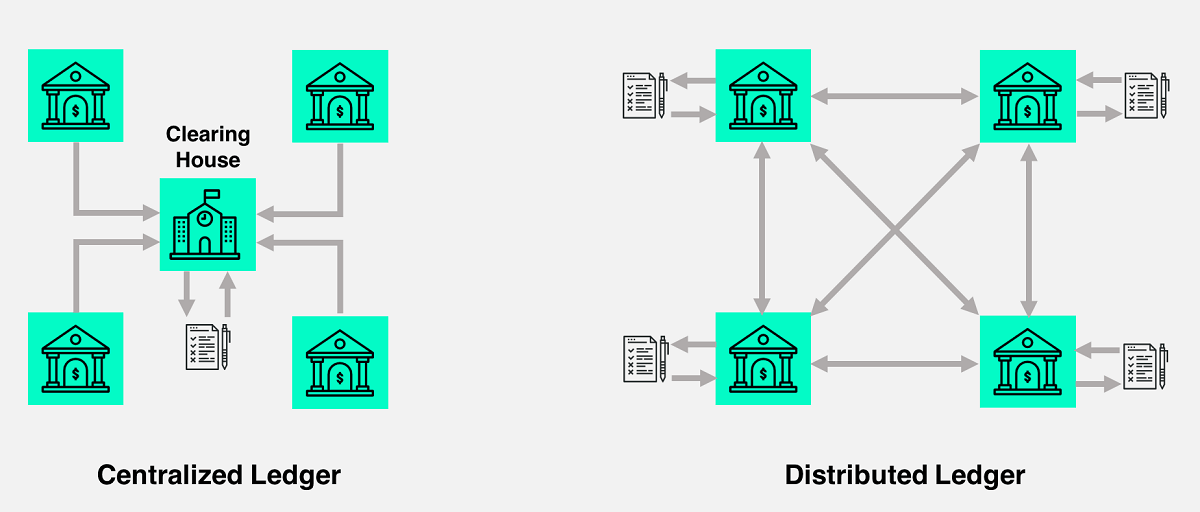
\includegraphics[width=\textwidth]{1.png}
\end{centerfig}

% Insert code
\begin{lstlisting}
  var a = 1;
  var b = 2;
  var c = a + b;
  console.log(c);
\end{lstlisting}

\begin{thebibliography}{9}
  \bibitem{sceta}
  \url{https://sceta.io/distributed-ledger-technologies}
 
\end{thebibliography}

\end{document}